\section{Differential Equations}
Differential equations involve variables and their derivatives. Unlike algebraic equations which evaluate to numbers or values, differential equations evaluate to a function of class of (several) functions.

\subsection{Modelling Differential Equations}
When interpreting words to model differential equations, there a few keywords that should be looked out for. They are listed below:
\begin{itemize}
	\item \textbf{Proportional:} means that the rate of change of a variable is equal to some constant $k$ multiplied by the another variable.

	A habitat of prairie dogs can support at most $m$ dogs. The habitat's population, $p$, grows proportionally to the product of the current population and $m - p$.

	The population's rate of change can be modelled using:
	\[ \frac{dp}{dt} = kp(m - p). \]

	\item \textbf{Shrinks, decays, melts, decreases, etc.:} any word that suggests something is getting smaller, the rate of change of a variable is negatively proportional to another variable.

	A radioactive material decays at a rate proportional the current amount, $Q$, of the material.

	The amount of material can be modelled using:
	\[ \frac{dQ}{dt} = -kQ. \]

	\item \textbf{Inversely Proportional:} the rate of change of a variable is equal to the inverse of another variable, multiplied by some constant $k$.

	A chemical is diluted out a tank by pumping pure water into the tank and pumping the existing solution out of it, so the volume at any time $t$ is $20 - 2t$. The amount $z$ of chemical in the tank decreases at a rate proportional to $z$ and inversely proportional to the volume of the solution in the tank.

	The rate of change of the amount of chemical in the tank can be modelled using:
	\[ \frac{dz}{dt} = -\frac{kz}{20 - 2t}. \]

	\item \textbf{Fraction of ... :} means that the rate of change of a variable is equal to some constant $k$ multiplied by one minus what the rate of change is proportional to.

	In one kind of chemical reaction, unconverted reactants change into converted reactants. The fraction $a$ of reactants that have been converted increases at a rate proportional to the product of the fraction of converted reactants and the fraction of unconverted reactants.

	The rate of change of the converted reactants can be modelled using:
	\[ \frac{da}{dt} = ka(1 - a). \]
\end{itemize}

\subsection{Slope Fields}
A slope field is a graphical representation of the solutions to a differential equation. They show all the different slopes of an equation at each point on a plane. For example, the slope field for the differential equation $\frac{dy}{dx} = \frac{x - 2}{y}$ is shown below:
\begin{figure}[H]
	\centering
	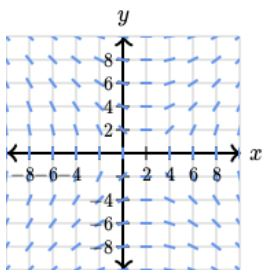
\includegraphics{images/fig13.JPG}
	\caption{A slope field.}
\end{figure}

We can confirm that this slope field visualizes the above equation by testing out a few points. For example:
\begin{itemize}
	\item At $(0, 0)$, $\frac{dy}{dx} = \frac{-2}{0}$, or undefined. This is seen in the slope field as a vertical line, matching the undefined slope.
	\item At $(2, 2)$, $\frac{dy}{dx} = \frac{0}{2}$. This is seen in the slope field by a horizontal line, matching the slope of $0$.
	\item At $(-6, 5)$, $\frac{dy}{dx} = \frac{-8}{5}$. This is seen in the slope field by a line with downwards slope, somewhat matching the slope of $-\frac{8}{5}$.
\end{itemize}

\subsection{Approximation Using Euler's Method}
Euler's method can use used to approximate solutions to differential equations. By solving for the slope, $\frac{dy}{dx}$, at one $x$ value, we can extend it to approximate the value of another $x$ on the function. At this next point, repeat the steps until we reach a specified $x$ value.

The general formula for approximating the next value of $f(x)$ given a differential equation and a change in $x$ ($\Delta x$) is given as:
\[ f(x_{n + 1}) = f(x_n) + \Delta x \cdot \frac{dy}{dx} \Big|_{x_n}. \]

\noindent \textbf{Examples:}
\begin{enumerate}
	\item Given $\frac{dy}{dx} = 2x - 3y$ and $f(-1) = 1$, approximate $f(3)$ using the Euler's method with $4$ equal steps of $\Delta x = 1$.

	The given point is at $(-1, 1)$. The slope at this point is:
	\[ \frac{dy}{dx} = 2(-1) - 3(1) = -5. \]

	Next, we can set up a table of what is given:
	\begin{table}[H]
		\centering
		\begin{tabular}{|c|c|c|c|}
			\hline
			$n$ & $x$ & $f(x)$ & $\frac{dy}{dx}$ \\
			\hline \hline
			$0$ & $-1$ & $1$ & $-5$ \\
			\hline
			$1$ & $0$ & ? & \\
			\hline
			$2$ & $1$ & & \\
			\hline
			$3$ & $2$ & & \\
			\hline
			$4$ & $3$ & & \\
			\hline
		\end{tabular}
	\end{table}

	To solve for the box marked by a `?', apply the formula.
	\begin{align*}
		f(x_{n + 1}) &= f(x_n) + \Delta x \cdot \frac{dy}{dx} \Big|_{x_n} \\[5pt]
		f(x_1) &= f(x_0) + \Delta x \cdot \frac{dy}{dx} \Big|_{x_0} \\[5pt]
		&= 1 + 1 \cdot (-5) \\
		f(x_1) &= -4.
	\end{align*}

	Repeat this process for the remaining missing squares. In the end the table should look like this:
	\begin{table}[H]
		\centering
		\begin{tabular}{|c|c|c|c|}
			\hline
			$n$ & $x$ & $f(x)$ & $\frac{dy}{dx}$ \\
			\hline \hline
			$0$ & $-1$ & $1$ & $-5$ \\
			\hline
			$1$ & $0$ & $-4$ & $12$ \\
			\hline
			$2$ & $1$ & $8$ & $-22$ \\
			\hline
			$3$ & $2$ & $-14$ & $46$ \\
			\hline
			$4$ & $3$ & $32$ & \\
			\hline
		\end{tabular}
	\end{table}

	Therefore, using Euler's method, we have concluded that $f(3) \approx 32$.

	\item Do the same problem as above but with $\Delta x = 2$.

	As with before, we can set up a table. But this time, there will only be two steps instead of $4$. It should look like this:
	\begin{table}[H]
		\centering
		\begin{tabular}{|c|c|c|c|}
			\hline
			$n$ & $x$ & $f(x)$ & $\frac{dy}{dx}$ \\
			\hline \hline
			$0$ & $-1$ & $1$ & $-5$ \\
			\hline
			$1$ & $1$ & ? & \\
			\hline
			$2$ & $3$ & & \\
			\hline
		\end{tabular}
	\end{table}

	To solve for the box marked by a `?', apply the formula:
	\begin{align*}
		f(x_{n + 1}) &= f(x_n) + \Delta x \cdot \frac{dy}{dx} \Big|_{x_n} \\[5pt]
		f(x_1) &= f(x_0) + \Delta x \cdot \frac{dy}{dx} \Big|_{x_0} \\[5pt]
		&= 1 + 2 \cdot (-5) \\
		f(x_1) &= -9.
	\end{align*}

	Repeat this process for the remaining missing squares. In the end the table should look like this:
	\begin{table}[H]
		\centering
		\begin{tabular}{|c|c|c|c|}
			\hline
			$n$ & $x$ & $f(x)$ & $\frac{dy}{dx}$ \\
			\hline \hline
			$0$ & $-1$ & $1$ & $-5$ \\
			\hline
			$1$ & $1$ & $-9$ & $28$ \\
			\hline
			$2$ & $3$ & $47$ & \\
			\hline
		\end{tabular}
	\end{table}

	Therefore, using Euler's method, we have concluded that $f(3) \approx 47$. Notice that by changing the value of $\Delta x$, the value and accuracy of the final approximation can change drastically.
\end{enumerate}

\subsection{Separable Differential Equations}
In a separable differential equation, the variables can be rearranged so that all the $x$'s are on one side, while all the $y$'s are on the other. Doing so makes it possible to separately integrate both sides of the equation.

Not all differential equations are separable. For an equation to be separable, it must be either the product or quotient of $f(x)$ and $g(y)$. For example, they may be in the form:
\[ \frac{dy}{dx} = f(x) g(y) \quad \text{or} \quad \frac{dy}{dx} = \frac{g(y)}{f(x)}. \]
Some more examples of both separable and non-separable differential equations are listed below:
\begin{enumerate}
	\item The equation: $\frac{dy}{dx} = 3x + 4y$ is not separable, as it is the sum of two functions.
	\item The equation: $\frac{dy}{dx} = 2^{x - y}$ is separable. It can be rearranged to be the product of $f(x)$ and $g(y)$ as follows:
	\[ 2^{x - y} = 2^x \cdot 2^{-y}. \]
	\item The equation: $\frac{dy}{dx} = 5y - x^2 y$ is separable. It can be rearranged to be the product of $f(x)$ and $g(y)$ as follows:
	\[ 5y - x^2 y = (5 - x^2) \cdot y. \]
\end{enumerate}

\subsubsection{General Solutions}
A general solution to a differential equation takes into consideration the entire class of possible solutions. This means that we have to add a constant $C$ to the end of the function. For example, find the general solution for the following differential equation:
\[ \frac{dy}{dx} = \frac{e^x}{y^2}. \]

\noindent The first step if to separate the equation. This means rearranging the equation into the form: $f(y) \; dy = g(x) \; dx$. Normally, it is considered unorthodox to separate $dx$ and $dy$, but in this case it is allowed. The equation then becomes:
\begin{align*}
	\frac{dy}{dx} &= \frac{e^x}{y^2} \\[5pt]
	y^2 \frac{dy}{dx} &= e^x \\[5pt]
	y^2 \; dy &= e^x \; dx.
\end{align*}

\noindent Next, take the integral of both sides. If the left and right sides are equal, then their Antiderivatives would also be equal.
\begin{align*}
	\int y^2 \; dx &= \int e^x \; dx \\[5pt]
	\frac{y^3}{3} &= e^x + C
\end{align*}

\noindent Notice that we only need to add a constant to one side, as adding it to both sides would be redundant. The final step is to rearrange the equation and solve for $y$. Note that in the second step, $3C = C$ because $3$ times a constant is still a constant.
\begin{align*}
	\frac{y^3}{3} &= e^x + C \\[5pt]
	y^3 &= 3e^x + 3C \\
	y^3 &= 3e^x + C \\
	y &= \sqrt[3]{3e^x + C}
\end{align*}

\subsubsection{Particular Solutions}
Particular solutions to differential equations have one answer. That is, we also have to solve for the value of the constant $C$. This is possible when given the value of $y$ at a point $x$. For example, find the particular solution to the following differential equation:
\[ f'(x) = \frac{16}{x^2} \quad \text{where} \quad f(-2) = 0. \]

\noindent The first step would be to find the general solution of $f(x)$.
\begin{align*}
	\frac{dy}{dx} &= \frac{16}{x^2} \\[5pt]
	dy &= \frac{16}{x^2} \; dx \\[5pt]
	\int 1 \; dy &= \int \frac{16}{x^2} \; dx \\[5pt]
	y &= -\frac{16}{x} + C
\end{align*}

\noindent To find the particular solution, we have to use $f(-2) = 0$. Substitute this into the general equation to solve for $C$.
\begin{align*}
	f(-2) &= 0 \\
	-\frac{16}{-2} + C &= 0 \\[5pt]
	C &= -8
\end{align*}

\noindent Therefore, the particular solution to the differential equation is:
\[ f(x) = -\frac{16}{x} - 8. \]

\subsection{Homogeneous Differential Equations}
A homogeneous differential equation is in the form $\frac{dy}{dx} = f \left( \frac{y}{x} \right)$. To solve these, we can make the substitution $v = \frac{y}{x}$. Through implicit differentiation with respect to $x$, we also get: $\frac{dy}{dx} = x \frac{dv}{dx} + v$.

\noindent Here is an example of a differential equation that can be solved using this method:
\[ 4x \frac{dy}{dx} = x + 2y. \]

\noindent First, by dividing both sides of the equation by $4x$, we can rewrite the right-hand side as a function of $\frac{y}{x}$:
\[ \frac{dy}{dx} = \frac{1}{4} = \frac{1}{2} \cdot \frac{y}{x}. \]

\noindent Next, we make the respective substitutions for $\frac{y}{x}$ and $\frac{dy}{dx}$:
\begin{align*}
	x \frac{dv}{dx} + v &= \frac{1}{4} + \frac{v}{2} \\[5pt]
	x \frac{dv}{dx} &= \frac{1}{4} - \frac{v}{2}.
\end{align*}

\noindent Now, we can solve the new differential equation with $v$ and $x$.
\begin{align*}
	x \frac{dv}{dx} &= \frac{1}{4} - \frac{v}{2} \\[5pt]
	x \frac{dv}{dx} &= \frac{1 - 2v}{4} \\[5pt]
	\frac{4}{1 - 2v} \; dv &= \frac{1}{x} \; dx \\[5pt]
	\int \frac{4}{1 - 2v} \; dv &= \int \frac{1}{x} \; dx \\[5pt]
	-2 \ln |1 - 2v| &= \ln |x| + C \\
	\ln |1 - 2v| &= -\frac{1}{2} \ln |x| + C \\[5pt]
	1 - 2v &= e^{-\frac{1}{2} \ln |x| + C} \\
	1 - 2v &= e^{-\frac{1}{2} \ln |x|} \cdot e^C
\end{align*}

\noindent At this point, $e^C$ is just another constant. Let this new constant be $A$.
\begin{align*}
	1 - 2v &= A e^{-\frac{1}{2} \ln |x|} \cdot e^C \\
	1 - 2v  &= A x^{-\frac{1}{2}} \\
	v &= \frac{1 - A x^{-\frac{1}{2}}}{2}
\end{align*}

\noindent Finally, substitute $\frac{y}{x}$ back into $v$.
\begin{align*}
	\frac{y}{x} &= \frac{1 - A x^{-\frac{1}{2}}}{2} \\[5pt]
	y &= x \left( \frac{1 - A x^{-\frac{1}{2}}}{2} \right)
\end{align*}

\subsection{Integrating Factor}
The integrating factor technique can be used to solve any differential equation in the form:
\[ \frac{dy}{dx} + P(x) y = Q(x). \]
By multiplying the equation by another function, $I(x)$, we notice that the left-hand side of the equation resembles the product rule for implicitly differentiating $I(x) y$:
\[ I(x) \frac{dy}{dx} + I(x) P(x)y = I(x) Q(x). \]
Therefore, we need to find $I(x)$ so that $I'(x) = I(x) P(x)$. This can be done by solving the differential equation with the following steps. Notice that the constant factor is not considered in the integrating step to simplify the final product.
\begin{align*}
	I'(x) &= I(x) P(x) \\
	P(x) &= \frac{I'(x)}{I(x)} \\[5pt]
	\int P(x) \, dx &= \int \frac{I'(x)}{I(x)} \, dx \\[5pt]
	\int P(x) \, dx &= \ln |I(x)| \\[5pt]
	I(x) &= e^{\int P(x) \, dx}
\end{align*}
Altogether, the steps for using the integrating factor technique are as follows:
\begin{enumerate}
	\item Calculate the integrating factor using $I(x) = e^{\int P(x) \, dx}$.
	\item Multiply both sides of the equation by $I(x)$.
	\item Integrate to obtain a general solution.
\end{enumerate}

\noindent \textbf{Examples:}
\begin{enumerate}
	\item Solve the following differential equation using the integrating factor technique:
	\[ \frac{dy}{dx} - 4y = e^x. \]

	First, we notice that $P(x) = -4$. Therefore:
	\begin{align*}
		I(x) &= e^{\int -4 \, dx} \\
		I(x) &= e^{-4x}
	\end{align*}

	Multiplying the differential equation by $I(x)$ gives:
	\[ e^{-4x} \frac{dy}{dx} - e^{-4x} \cdot 4y = e^x \cdot e^{-4x}. \]

	Finally, we can solve for the general solution.
	\begin{align*}
		e^{-4x} \frac{dy}{dx} - e^{-4x} \cdot 4y &= e^x \cdot e^{-4x} \\[5pt]
		\frac{d}{dx} \left( e^{-4x}y \right) &= e^{-3x} \\[5pt]
		\int \frac{d}{dx} \left( e^{-4x}y \right) \, dx &= \int e^{-3x} \, dx \\[5pt]
		e^{-4x}y &= -\frac{e^{-3x}}{3} + C \\[5pt]
		y &= -\frac{e^x}{3} + C e^{4x}
	\end{align*}

	\item Solve the following differential equation using the integrating factor technique:
	\[ x^2 \frac{dy}{dx} + 2xy = 1. \]

	Immediately, we observe that the equation is already in the form $I(x) \frac{dy}{dx} + I(x) P(x)y = I(x) Q(x)$, with $P(x) = 2x$:

	Thus, we can solve this by integrating both sides:
	\begin{align*}
		\frac{d}{dx} \left( x^2 y \right) &= 1 \\[5pt]
		\int \frac{d}{dx} \left( x^2 y \right) \, dx &= \int 1 \, dx \\[5pt]
		x^2 y &= x + C \\
		y &= \frac{x + C}{x^2}
	\end{align*}
\end{enumerate}

\subsection{Exponential Model Equations}
An exponential equation involves a function whose derivative is proportional to itself. It is usually in the form $f(x) = C \cdot a^x$, where $C$ and $a$ are both constants.

\noindent \textbf{Examples:}
\begin{enumerate}
	\item Solve for $g(x)$, given $g'(x) = -4 g(x)$ and $g(-2) = 12$.

	The first step is to find a general solution for $g(x)$:
	\begin{align*}
		g'(x) &= -4 g(x) \\
		\frac{dy}{dx} &= -4y \\[5pt]
		\frac{1}{y} \; dy &= -4 \; dx \\[5pt]
		\int \frac{1}{y} \; dy &= \int -4 \; dx \\[5pt]
		\ln |y| &= -4x + C \\
		y &= e^{-4x + C} \\
		y &= A e^{-4x}.
	\end{align*}

	Next, we solve for the constant $A$ using $g(-2) = 12$, to find the particular solution for $g(x)$:
	\begin{align*}
		g(-2) &= 12 \\
		A e^{-4 \cdot (-2)} &= 12 \\
		A e^8 &= 12 \\
		A &= 12 e^{-8}.
	\end{align*}

	Putting everything together:
	\[ g(x) = 12 e^{-8} \cdot e^{-4x} = 12 e^{-4x - 8}. \]

	\item The number of barrels of oil a certain company exports annually increases at a rate that is proportional at any time to the number of barrels they export at that time. The company exported $5.4$ million barrels annually initially, and it exported $10.8$ million barrels annually after $6$ years. \textbf{How many million barrels of oil did the company export after $10$ years?}

	First, we can model the differential equation. Let $B$ be the number of millions of barrels of oil, and $t$ be the time in years. The rate of change of barrels is proportional to the number of barrels, so:
	\[ \frac{dB}{dt} = kB \]
	for some constant $k$.

	Let $B(t)$ be the function that represents the number of barrels exported at time $t$. From the question, we are given:
	\[ B(0) = 5.4 \quad \text{and} \quad B(6) = 10.8. \]

	Thus, we can first solve for a general solution to $B(t)$:
	\begin{align*}
		\frac{dB}{dt} &= kB \\[5pt]
		\frac{1}{B} \; dB &= k \; dt \\[5pt]
		\int \frac{1}{B} \; dB &= \int k \; dt \\[5pt]
		\ln |B| &= kt + C \\
		B(t) &= e^{kt + C} \\
		B(t) &= A e^{kt}.
	\end{align*}

	Using the two given points of data, we can solve for $A$ and $k$ to find the particular solution:
	\begin{align*}
		B(0) &= 5.4 \\
		A e^{0k} &= 5.4 \\
		A &= 5.4 \\[12pt]
		B(6) &= 10.8 \\
		5.4 e^{6k} &= 10.8 \\
		e^{6k} &= 2 \\
		6k &= \ln 2 \\
		k &= \frac{\ln 2}{6}.
	\end{align*}

	Putting everything together:
	\[ B(t) = 5.4 e^{\frac{\ln 2}{6} t} = 5.4 \cdot 2^{\frac{t}{6}}. \]

	Thus, in $10$ years, the company will be making $B(10) \approx 17$ million barrels of oil.
\end{enumerate}

\subsection{Logistic Growth Model Equations}
A logistic growth model is an s-shaped curve that starts by growing rapidly before slowing down as it approaches its \textit{carrying capacity}.

One application of the logistic growth model is in modelling population. The change in population is proportional to the product of the population at the time, $P$, and the difference between $1$ and the population over the carrying capacity, $C$. The differential equation for this is:
\[ \frac{dP}{dt} = kp \left( 1 - \frac{P}{C} \right). \]

\begin{figure}[H]
	\centering
	\frame{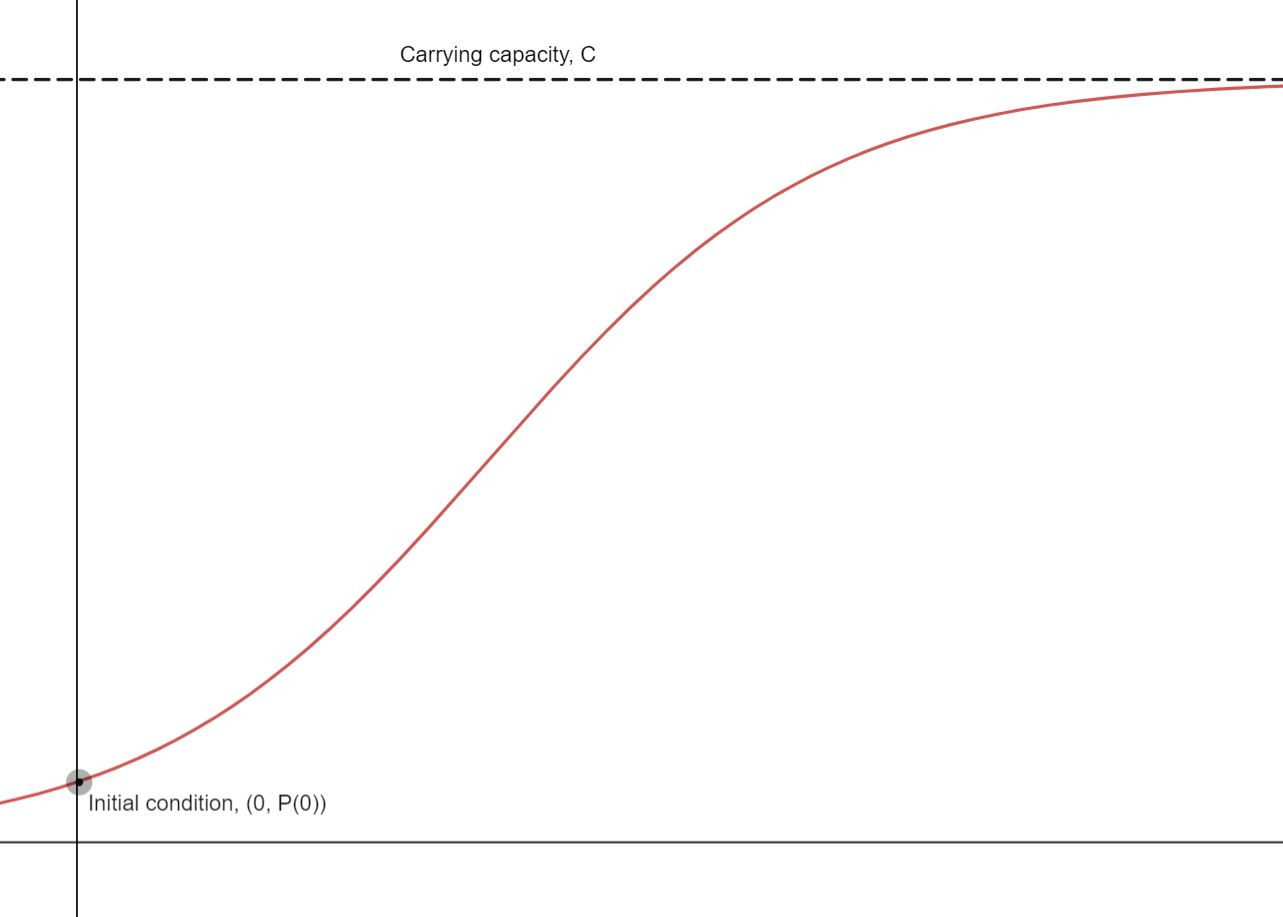
\includegraphics[width=0.6\textwidth]{images/fig14.JPG}}
	\caption{Logisitic equation, $P(t)$.}
\end{figure}

\noindent \textbf{Examples:}
\begin{enumerate}
	\item Find the carrying capacity of the following logistic growth:
	\[ \frac{dP}{dt} = \frac{1}{50} P (35000 - P). \]

	For any logistic model $P$, the rate of change $\frac{dP}{dt}$ will be $0$ at the carrying capacity (the population stops growing).
	\begin{gather*}
		\frac{dP}{dt} = 0 \\[5pt]
		\frac{1}{50} P (35000 - P) = 0 \\[5pt]
		P = 0, \; 35000
	\end{gather*}

	$P = 0$ is at the start of the model, so $P = 35000$ is the carrying capacity.

	\item At what value $N$ does the following logistic model grow the quickest?
	\[ \frac{dN}{dt} = N \left( 1 - \frac{N}{180} \right) \]

	The point at which the logistic model grows the quickest is when the derivative changes from increaseing to decreasing. This is at its point of inflection. Recall that the point of inflection occurs when the second derivative equals $0$, or when $\frac{d^2 N}{dt^2} = 0$.

	First, find the second derivative:
	\begin{align*}
		\frac{dN}{dt} &= N \left( 1 - \frac{N}{180} \right) \\[5pt]
		\frac{dN}{dt} &= N - \frac{N^2}{180} \\[5pt]
		\frac{d^2 N}{dt} &= 1 - \frac{N}{90}.
	\end{align*}

	Next, find the point of inflection by setting $\frac{d^2 N}{dt} = 0$:
	\begin{align*}
		\frac{d^2 N}{dt} &= 0 \\[5pt]
		1 - \frac{N}{90} &= 0 \\[5pt]
		N &= 90
	\end{align*}

	Therefore, the model is growing the quickest at $N = 90$.
\end{enumerate}
